%!TEX root = report.tex

The final assignment used the code from the second assignment as basis, but a different dataset. The CIFAR-10 dataset was used, a dataset with 10 distinct classes such as airplane, dog or frog.

\subsection*{Input}
A different dataset meant that the format of the images also was different. The previous MNIST dataset used gray scale images which are 28 by 28 digits, while the CIFAR-10 dataset used colour images which are 32 by 32 pixels. 

Therefore the data first had to be reshaped in order to be able to be parsed by the neural network. The size of the filter also had to be changed, as well as the kernel sizes had to be increased from 4x4 to 5x5.

The dataset was split into six batches, five training batches and one test batch. For ease of use is the fifth training batch used as validation set, giving us a balanced training/validation/test set.
\todo{example images}

\subsection*{Architecture}
\todo{parameters}
A number of settings for the neural network were tested in order to see which architecture gave the best scores. The size of nodes per hidden layers, the amount of hidden layers and amount of kernels were varied in order to see which gave the best result.

One of the issues we came across was a problem of overfitting. One of the methods to reduce overfitting available is to use dropout \cite{srivastava2014dropout}. For each hidden layer used, a random mask of ones and zeroes is made and multiplied with the output of the layer. This randomly disables nodes while training in a hidden layer, preventing local optima \todo{check truth}.

The results obtained are using two almost equal architectures. The main difference between the two is that one uses local contrast normalization, while the other does not.

The architecture is as follows: first the image goes into the first convolution layer with 32 kernels, where the image is filtered and reduced from 32 by 32 to 14 by 14. The second convolution layer has 64 kernels and reduces the image size even further to a shape of 5 by 5. \todo{cite/read the paper} 

This is flattened and then sent to the first hidden layer with rectified linear units. This has 1600 inputs and reduces the data to 1250 outputs. The second hidden layer also uses rectified linear units and reduces the data further, from 1250 inputs to 128 outputs. 

Finally the output layer consists of logistic regression, which has ten potential outputs for each of the classes.

\subsection*{Results}
The results are presented in a graph, showing the change in the training, validation and test error over the epochs. Furthermore is there a graph with all of the kernels visualized. The results from two full runs are shown, one with local contrast normalization and one without. This allows us to also compare the effects of having local contrast normalization.

\begin{figure}[ht!]
	\centering
	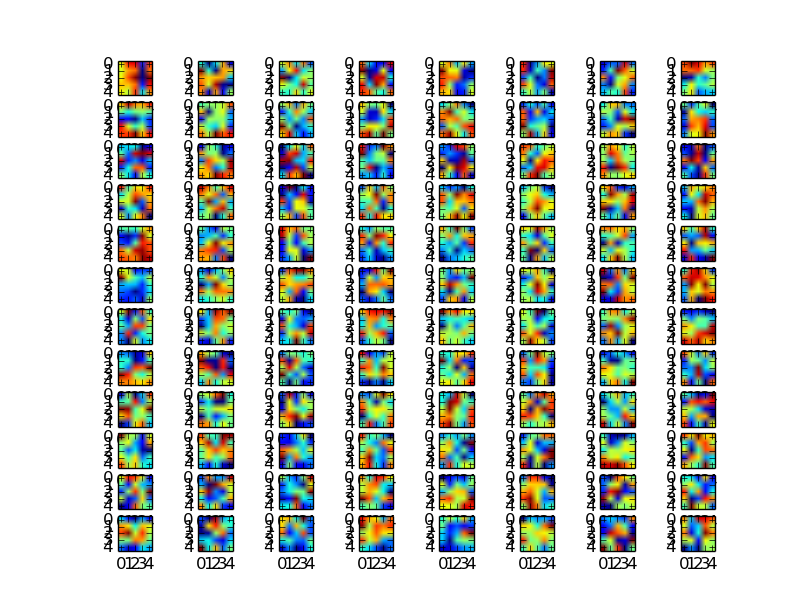
\includegraphics[width=0.9\textwidth]{./img/Exercise3/Run1/3264end.png}	
	\caption{The kernels for a run without LCN.}
	\label{fig:3:kernelsNoLCN}
\end{figure}

\begin{figure}[ht!]
	\centering
	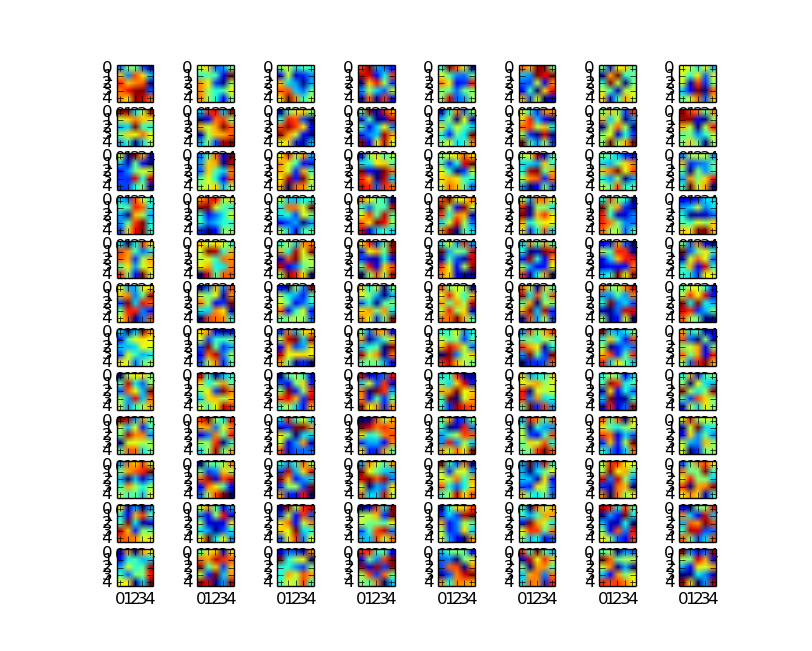
\includegraphics[width=0.9\textwidth]{./img/Exercise3/Run2LCN/ass3final.png}	
	\caption{The kernels for a run with LCN.}
	\label{fig:3:kernelsLCN}
\end{figure}


\todo{error graphs}]
Runtime: 34.13 minutes when not using LCN.
